\documentclass{article}
\usepackage[T1]{fontenc}
\usepackage{lmodern}
\usepackage{graphicx}
\usepackage{amsmath,amssymb}
\usepackage[a4paper,margin=2cm]{geometry}
\usepackage[absolute,overlay]{textpos}
\setlength{\TPHorizModule}{1mm}
\setlength{\TPVertModule}{1mm}
\usepackage[indonesian]{babel}
\usepackage{hyperref}
\setlength{\emergencystretch}{2em}
% unit: Halaman 74

\begin{document}

% === Halaman 74 (llm) ===

\vspace{278.29mm}

\begin{verbatim}
import numpy as np
from PIL import Image

def EmbeddingPesan(cover, pesan, stego):
    # Baca citra cover, ekstrak pixel-pixel sebagai sebuah larik (array)
    citra = Image.open(cover, 'r')
    citra = citra.convert("RGB")
    n = 3
    citra.show()
    lebar, tinggi = citra.size
    larik_pixel = np.array(list(citra.getdata()))

    total_pixel = larik_pixel.size//n    #jumlah pixel di dalam citra
    pesan = pesan + "#####"    #tambahkan delimiter '#####' untuk menandai akhir pesan

    #ubah pesan menjadi string biner
    pesan_biner = ''.join((format(ord(i), "08b") for i in pesan))
    panjang_bit_pesan = len(pesan_biner)

    # periksa apakah jumlah pixel di dalam citra mencukupi untuk menyisipkan pesan
    if panjang_bit_pesan > total_pixel:
        print("ERROR: Ukuran citra tidak mencukupi untuk penyembunyian pesan")
    else:
\end{verbatim}

% deskripsi: Screenshot kode program Python untuk fungsi EmbeddingPesan menggunakan pustaka numpy dan PIL untuk steganografi citra.
% bbox normalisasi: [0.0470, 0.0300, 0.9420, 0.9670]
\begin{textblock*}{187.95mm}(9.87mm,8.91mm)
\noindent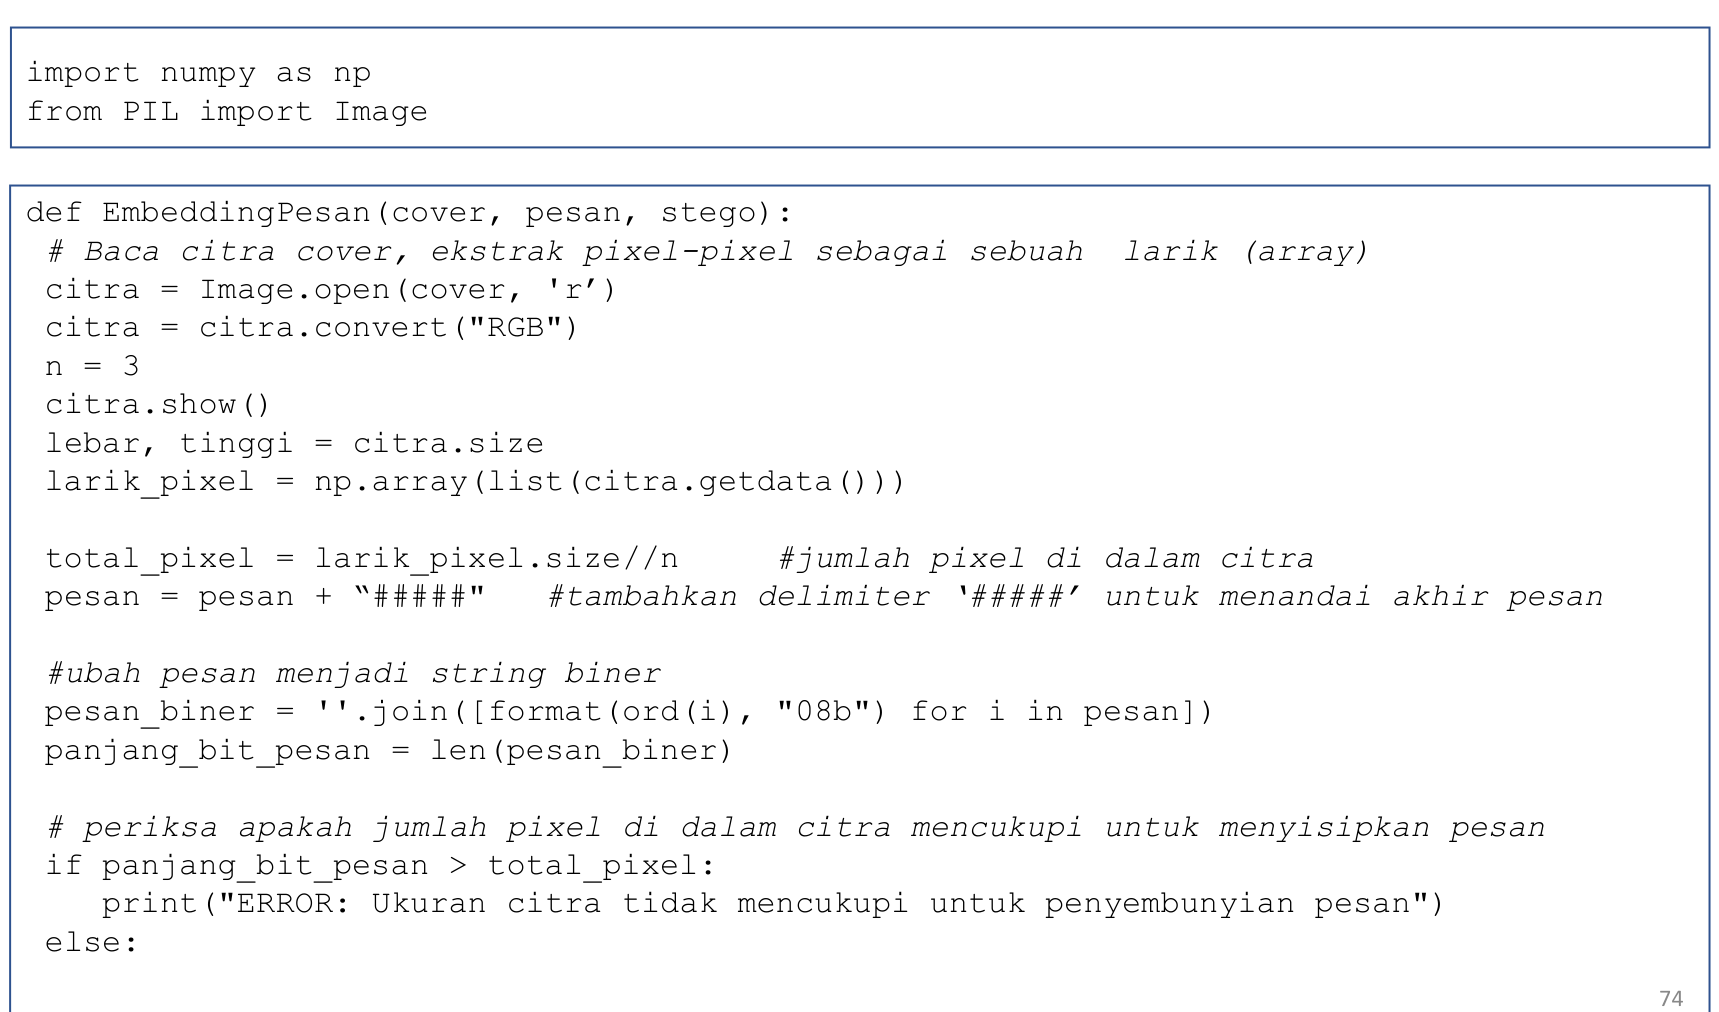
\includegraphics[width=187.95mm,height=278.29mm]{../../images/llm/page_074_img_01.png}%
\end{textblock*}

\end{document}
